\chapter{相关算法及Hadoop分布式数据处理}
本文提出的推荐系统基于语义分析、协同过滤算法、Hadoop和MapReduce等几个基本算法及基本概念。
以下简单介绍这几个算法及概念。

\section{语义分析}
字、词是自然语言中最重要的一种独立、有意义的元素。
一句话离不开字、词,整句话的意思也由字、词的独自意思组合变形而成。
亚洲语言,特别是中文,它们和拉丁语言,如英语、西班牙语,之间有巨大的差异,
因为亚洲语言缺少界定符号来标定字、词的边界,同时许多亚洲语言的字、词没有特定的,明确的意思。
在中文语言处理中,最基础的工作是划分字、词,也就是把汉语句子划分成一连串的字词,
因为,这是自然语言处理接下来的工作,如词义类型标记、语法分析等,的基础。
为了从用户上网流量记录中分析用户的兴趣爱好,我们需要通过语义分析的方法对用户曾经浏览过网页的内容进行提取、标记和分类。
语义分析包含以下主要步骤:
\begin{enumerate}
	\item 句尾检测

	这一步主要是把一段文字分成一个有意义句子的集合\parencite{kiss2006unsupervised}。
	因为句子一般都含有思想的逻辑单元,所以句子的语法是可以预测的。
	而切词工作是建立在单个句子上的,所以分析文章一般从句尾检测开始。
	
	\item 切词
	
	这一步主要在单个句子上进行操作,将句子分为单个词。
	切词工作对于不同的文字有不同的切法,比如英文切词工作主要按空格切分,但还要注意不能混淆点号的意义;
	而中文没有空格,切词时要按照语料库是否存在该词来切分。

	\item 词义类型标记

	这一步主要是在切好的词语中标记词语的类型,比如是动词还是名词或者是长名词中的一部分。
	对于社交网络中的语言,比如推特或者微博,语言比较口语化,会出现大量动词名词混用情况\parencite{Gimpel2011Part,Owoputi2015Improved,Derczynski2013Twitter}。
	通过标记,机器甚至能指出名词或者是长名词是属于什么类型,比如是人,地点,或者组织。
	
	\item 分块
	
	这一步主要是在有逻辑意义的整句和复合标记的基础上分析词语。
	根据预先定义好的语法,将标记了类型的词语分成块。

	\item 提取主要内容

	这一步主要是进一步为分好的块标记名称或者类型,这与第三步词义类型标记不同,因为这一步以块为整体标记名称或者类型。
\end{enumerate}

其中每一步都很关键,因为一旦其中一步出错,误差会逐步传播,使得语义分析出严重错误。语义分析可以用经典的F1 score来计算其准确程度。下面简单介绍计算F1 score方法。在语义分析完成后,统计以下数量:
\begin{center}
\begin{itemize}
	\item $TP$:被正确识别为实体的词语
	\item $FP$:本来不应该被正确识别为实体的但确实被正确识别为实体的词语
	\item $TN$:本来不应该被正确识别为实体的,同时没有被正确识别为实体的词语
	\item $FN$:本来应该被正确识别为实体的,但没有被正确识别为实体的词语
\end{itemize}
\end{center}
此时再定义精确度$precision$与召回率$recall$如下:
\begin{equation}
precision= \frac{TP}{TP+FP}
\end{equation}
\begin{equation}
recall= \frac{TP}{TP+FN}
\end{equation}
则可以用下式来描述语义分析模型的准确度为
\begin{equation}
F= 2* \frac{precision*recall}{precision+recall}
\end{equation}


\section{Hadoop和MapReduce}
随着互联网的发展,用户与物品间交互的数据越来越多,基于单个机器的推荐系统的处理效率和可扩展性已经开始阻碍极速增长的数据的快速处理。

在生产环境中,运行一个推荐系统所必需的离线计算必须遵守严格的时间和资源的限制,同时这又是更大的分析流程中的一部分,所以其必须定期被执行。
此外,必须通过重复运行推荐系统,以在交叉验证集中寻找良好模型参数。
但这在经济上和操作上往往又是不可取的,因为在一台机器上执行这种离线计算十分有可能会失败。
并且面对着不断增长的数据量,要不断进行硬件升级来提高机器的性能,以满足时间上的限制。
正是由于这些缺点,使用单台机器运行推荐系统变得昂贵并且难以操作。
而在多个机器组成的集群上运行推荐系统,既能提高容错水平,又能解决数据密集的问题。
而Hadoop和MapReduce正是保存大数据以及并行处理数据的的最佳选择。

Hadoop由多个部分组成,其最基础的组件是Hadoop分布式文件系统(HDFS)。
HDFS的运行机制是把要写入的数据分发到大量计算机集群中,仅一次写入,就可以多次读取用于分析。
但它与其它分布式系统相比,最大的区别是不能删除,只能进行格式化。
\def\HDFSfront{
	\path (0,0) node(Splitn) [rectangle,draw] {Split(n)}
			(0,1) node {$\cdots$}
			(0,2) node(Split3) [rectangle,draw] {Split(3)}
			(0,3) node(Split2) [rectangle,draw] {Split(2)}
			(0,4) node(Split1) [rectangle,draw] {Split(1)}
			(0,5.5) node {\textbf{HDFS}};
	\draw (-1,-1) rectangle (1,6);
}
\def\HDFSend{
	\path (10,0) node(Partn) [rectangle,draw] {Part(n)}
			(10,1) node {$\cdots$}
			(10,2) node(Part3) [rectangle,draw] {Part(3)}
			(10,3) node(Part2) [rectangle,draw] {Part(2)}
			(10,4) node(Part1) [rectangle,draw] {Part(1)}
			(10,5.5) node {\textbf{HDFS}};
	\draw (9,-1) rectangle (11,6);
}
\def\mapper{
	\path (3.5,-1) node(Mapper4) [rectangle,draw] {\textbf{Mapper}}
			(3.5,0.5) node {$\cdots$}
			(3.5,2) node(Mapper3) [rectangle,draw] {\textbf{Mapper}}
			(3.5,3.5) node(Mapper2) [rectangle,draw] {\textbf{Mapper}}
			(3.5,5) node(Mapper1) [rectangle,draw] {\textbf{Mapper}};
}
\def\reducer{
	\path (7,1) node(Reducer2) [rectangle,draw] {\textbf{Reducer}}
			(7,2.5) node {$\cdots$}
			(7,4) node(Reducer1) [rectangle,draw] {\textbf{Reducer}};
}
\begin{center}
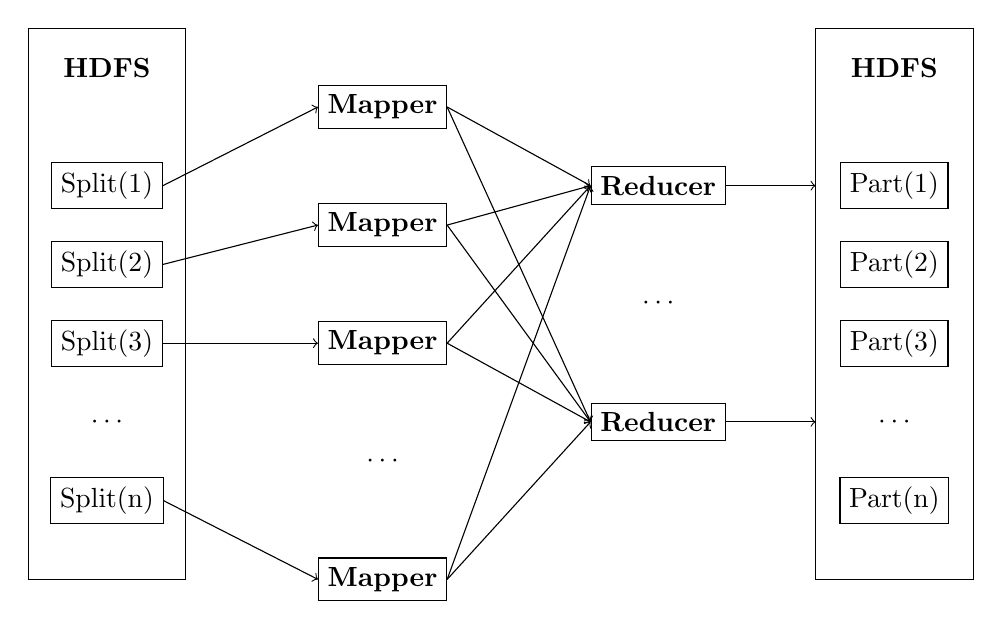
\begin{tikzpicture}
\HDFSfront
\mapper
\reducer
\HDFSend
\draw[->] (Split1.east) -- (Mapper1.west);
\draw[->] (Split2.east) -- (Mapper2.west);
\draw[->] (Split3.east) -- (Mapper3.west);
\draw[->] (Splitn.east) -- (Mapper4.west);
\draw[->] (Mapper4.east) -- (Reducer1.west);
\draw[->] (Mapper4.east) -- (Reducer2.west);
\draw[->] (Mapper3.east) -- (Reducer1.west);
\draw[->] (Mapper3.east) -- (Reducer2.west);
\draw[->] (Mapper2.east) -- (Reducer1.west);
\draw[->] (Mapper2.east) -- (Reducer2.west);
\draw[->] (Mapper1.east) -- (Reducer1.west);
\draw[->] (Mapper1.east) -- (Reducer2.west);
\draw[->] (Reducer1.east) -- (9,4);
\draw[->] (Reducer2.east) -- (9,1);
\end{tikzpicture}
\figurecaption{Hadoop的MapReduce工作流程图}
\label{fig:HadoopMapReduce}
\end{center}

Hadoop集群由一个主机和多个从机组成。
其中,主机是最重要的,它保持整个HDFS文件系统的正常运行,同时保持与每台从属机器的心跳连接。
HDFS中存储的文件被划分为的固定大小的存储块。
当文件被放置在HDFS时,主机将分配给每个存储块不同的全局标签。
为了保证数据的可靠性,每个存储块被多次复制,然后保存到不同的从机中去。
由于主机保持整个HDFS文件系统的正常运行,所以主机保存每个存储块的全局标签,并保存存储块的地址,还保存存储块和原始文件之间的映射关系。

通常Hadoop集群只有一台主机,这不仅简化大型机管理策略,同时也给主机整个系统全局信息,以方便储存和安置存储块。
有时上述HDFS除了有一个主机以外,还有一个影子主机,它缓存了主机的运行信息,这种设计使得它很容易从操作故障中重新启动并恢复。

Hadoop的主要执行框架即MapReduce。
对于保存在分布式文件系统的数据,MapReduce在每个数据节点上,获取本地的数据副本,然后进行本地运算。

图\ref{fig:HadoopMapReduce}为Hadoop的MapReduce工作流程图。
从该图中可以发现,MapReduce框架包含两个阶段,map阶段和reduce阶段。
输入数据和计算后的输出数据都是一个(key,value)集合。
用$<k,v>$来表示这些键值对。
key主要用在reduce阶段,用来决定哪个value结合在一起。
用两个函数来表示这两个过程:
\begin{eqnarray}
\mathbf{Mapper} &:& <k1,v1> \rightarrow list<k2,v2> \\
\mathbf{Reduce} &:& <k2,list<v2>> \rightarrow list<k3,v3>
\end{eqnarray}

计算过程从map阶段开始,在该阶段中,各从机接受主机的分配,然后同时地、并行地执行map函数。
此时保存在分布式文件系统的输入数据将被切分成很多个部分。
进行每次切分的同时主机就会对从机指定一个map任务。
在map阶段的后期,每个map函数的输出键值对将会对map函数中生成的键进行哈希分区。
紧接着进入reduce阶段。
在reduce阶段的初期,每个分区中的键值对将基于键分别排序,接着按照键的排序进行合并。
有同样的键的分区将被分配到同一个reduce任务中。
最后,在reduce阶段的后期,reduce函数输出键值合并的最终结果。

在Hadoop的MapReduce工作流程中,一个工作记录服务器作为主节点把数据分成几部分作为map阶段的输入。
同时任务记录服务器作为数据节点保存map函数中间生成的结果到HDFS中。

Hadoop集群对组成集群的计算机性能要求不高,所以即使古老的、配置低的服务器也能作为集群的一部分。
Hadoop会基于地点计划分配MapReduce运算,同时提高集群整体的输入输出效率来减少运算的成本。
这种工作方式将原本单独机器的运算工作合理地分配到多个机器中,不仅提高了数据运算的可靠性,还大大地提高了运算的效率。


\section{基于用户历史的协同过滤算法}
协同过滤算法基于三个假设:人们有共同的兴趣爱好;他们的兴趣爱好是稳定的;可以根据兴趣爱好的历史数据预测用户的选择。
协同过滤算法主要比较用户之间的行为,找到最近的相邻用户,根据最近的相邻用户的行为预测用户的兴趣爱好。

对于$m$个用户的用户集$U$,和$n$个物品的物品集$I$,用户$u_i \in U$与物品$i_j \in I$的交互信息记录为一个数值$r_{ij} \in R$。
若用户$i$对物品$j$无交互行为,则$r_{ij}=?$。
最基本的协同过滤算法所研究的问题为:基于$R$,给每位用户推荐一个不包含该用户已经评价过物品的列表,其中的物品按照符合用户兴趣程度递减排序。

协同过滤算法能分为主要两个步骤:第一步是计算用户$x$与用户$y$之间的相似程度:
\begin{equation}
S_{x,y} = \frac{\sum_{i\in I_{xy}}(r_{x,i}-\bar{r}_x)(r_{y,i}-\bar{r}_y)}{\sqrt{\sum_{i\in I_{xy}}(r_{x,i}-\bar{r}_x)^2}\sqrt{\sum_{i\in I_{xy}}(r_{y,i}-\bar{r}_y)^2}}
\end{equation}
其中$r_{x,i}$为用户$x$对物品$i$的评分,$\bar{r}_x$是用户$x$的平均评分,$I_{xy}$为与用户$x$和用户$y$曾发生交互行为的物品集。

第二步计算用户$u$对物品$i$评分的预测值$r_{u,i}$:
\begin{equation}
r_{u,i} = \bar{r}_u + \frac{\sum_{u'\in U^k}(r_{u',i}-\bar{r}_{u'})S_{u,u'}}{\sum_{u'\in U^k}S_{u,u'}}
\end{equation}
其中$U^k$为与用户$u$距离最近的$n$个用户。
最后,只需从物品集中筛选出预测分数前几的物品,推荐给用户$u$。
以上被称作基于用户的协同过滤算法,其中从以下几个方面,可以看出它是从用户的角度来工作的:
\begin{itemize}
\item 首先在计算相似度的时候,它是计算两个用户之间的相似度,这与基于物品的协同过滤算法正好相反,后者是计算两个物品之间的相似度;
\item 在计算评分的预测值之后,对每位用户的商品评分进行高低排序,然后推荐给用户排前几名的物品。
这与基于物品的协同过滤算法正好相反,后者是对每位商品的用户评分进行高低排序,而评分相对高的用户正是最有可能对该物品感兴趣的人。
\end{itemize}

就如上面所提到的,基于物品的协同过滤算法要先计算物品之间的相似度,得到物品的相似度矩阵。
然后在相近的物品之间计算用户可能评价的评分。
基于物品的协同过滤算法与基于用户的协同过滤算法基本上是一样的,其中最大的区别是其计算的顺序不同,一个更多使用User-Item矩阵的行,另一个更多使用User-Item矩阵的列。

但是,User-Item的行数与列数不同,会对这两种算法的性能有很大影响,特别是在单个机器上执行算法的时候。
如果用户数远远大于物品数,此时如果使用基于用户的协同过滤算法,计算的用户相似度矩阵就会很大,即很多行(相似度矩阵的行与列相等)。
相反,如果使用基于物品的协同过滤算法,计算的物品相似度矩阵就比较小。两种算法对于单个机器的固定内存大小来说尤其重要,因为相似度矩阵过大,有可能超过内存大小,或者占用过多内存使接下来的计算变慢。

以上两种算法都称作基于历史数据的协同过滤算法,因为他们都使用了用户与物品间交互的历史数据。
基于历史数据的协同过滤算法存在两个缺点:
\begin{itemize}
\item 在计算用户之间、物品之间的相似度矩阵时,时间复杂度为平方级别,即计算成本很高;
\item 推荐算法的精度取决于所用的相似度计算函数。如果没有按照用户与物品间历史交互数据选择合适的相似度计算函数,推荐算法的效果会不太理想。
\end{itemize}

\section{基于模型的协同过滤算法}
为了解决上面的问题,新的协同过滤算法被提出来,比如基于模型的协同过滤算法。
与基于历史数据的协同过滤算法不同的是,基于模型的协同过滤算法首先从User-Item矩阵中训练出一个模型,
然后以这个模型再进行计算,推荐物品给用户。
这个模型可以用公式描述:
\begin{equation}
f(p_i,q_j)\rightarrow R_{i,j},i=1,2,\dots M, j=1,2,\dots N
\end{equation}
其中$p_i$和$q_j$代表用户$i$和物品$j$的一对模型参数,$f$是把模型参数映射到已知的User-Item矩阵数据的一个模型参数。
所以基于模型的协同过滤算法的主要任务就是在模型函数$f$下,通过已知的User-Item矩阵数据$R_{i,j}$,预测参数$p_i$和$q_j$。

在众多的基于模型的协同过滤算法中,潜在因子模型运行性能突出,因为它解决了协同过滤算法中最常见的两个问题:
\begin{itemize}
\item User-Item矩阵过于稀疏,使得矩阵之间的运算时间、空间复杂度高;
\item User-Item矩阵虽然行列众多,但是其秩非常低,也就是说在这个User-Item二维空间中,许多信息是重合的,冗余的。
\end{itemize}

下面就来说明潜在因子模型的运行规则。
令$R$为$|C|\times|P|$的User-Item矩阵,其中包含了用户与物品间交互的历史信息。
$C$代表用户集,$P$代表了物品集。
如果用户$i$曾经与物品$j$间有交互动作发生,并产生了某个值$r_{i,j}$,代表着这个交互动作的强度。
潜在因子模型就是把$R$渐近地分解为两个秩为$r$的特征矩阵$U$和$M$,使得$R\approx UM$。
$|C|\times r$的矩阵$U$代表用户集的潜在因子,即$R$的行向量。
$r\times |P|$的矩阵$M$代表物品集的潜在因子,即$R$的列向量。
而用户和物品之间的交互强度的预测值可以在低维的矩阵空间中进行,即$u_i^Tm_j$,其中$u_i$是代表用户$i$的向量,$m_j$是代表物品$j$的向量。
所以,接下来的主要问题就是计算矩阵$U$和矩阵$M$。

比较常见的算法是随机梯度下降算法,即随机选取矩阵$U$和矩阵$M$的初始值,然后计算$u_i^Tm_j$与$r_{i,j}$之间的误差,通过迭代的方式顺着梯度最大方向下降而得出最优解。
\begin{equation}
U^*,M^* = \mathop{\argmax}_{U,M} \{\frac{1}{2} \sum_{i=1}^C \sum_{j=1}^P I_{i,j}(r_{i,j}-u_i^{\tau} u_j)^2 + \frac{\lambda_U}{2}\lVert U\rVert_F^2 +\frac{\lambda_M}{2}\lVert M\rVert_F^2\}
\end{equation}
其中$U^*$和$M^*$代表最小化运算后的最优解,$I_{i,j}$代表示性函数,即当其自变量大于零,函数值为一。

另外一种计算方法称为交替最小方差算法。
给定一个阈值$\epsilon$,通过以下步骤找到矩阵$U$和$M$:
\begin{enumerate}
	\item 随机选择一个矩阵$M$;
	\item 固定矩阵$M$,优化矩阵$U$;对逐个用户$u_i$进行优化,即固定$m_j$,需要找到
	\[
	\mathop{\argmax}_{u_i} \sum_{j\in R_i}(r_{i,j}-u_i\cdot v_j)^2
	\]
	这是线性最小二乘方程,可以得到
	\[
	u_i=(M_{*,i}^{\tau}M_{*,i})^{-1}M_{*,i}R_{*,i}
	\]
	其中$M_{*,i}$是有来自用户$u_i$的评价的$M$的子集。
	\item 固定矩阵$U$,优化矩阵$M$,与上一步相似;
	\item 循环第2、3步,直到相关系数的变化量小于$\epsilon$,即可得到收敛解。
\end{enumerate}

对比以上两种计算方法,我们可以发现,对于单个机器而言,随机梯度下降算法更适合于低阶矩阵因子化的计算。
这是因为随机梯度下降算法相比于交替最小方差算法更容易实现,并且前者计算量相对来说更小。

但是,随机梯度下降算法是序列算法,因为它在每次迭代后都要更新模型的参数。
而交替最小方差算法相比于随机梯度下降算法的优点在于,前者可以运用于并行计算。

虽然交替最小方差算法的计算量比随机梯度下降算法的计算量大得多,但是它的交替迭代方式让他更适用于并行计算。
例如,当我们计算用户特征矩阵$U$时,$U$的第$i$行$u_i$能同时用于解一个最小二乘方程,这个最小二乘方程中只包含$R$的第$i$行$r_i$,即用户$i$的交互信息,以及对应于$r_i$中不为零的位置的矩阵$M$中的所有列$m_j$。
$u_i$的同时重复使用是与矩阵$U$中其它行的计算相互独立的,所以矩阵$U$的计算很容易实现并行化,只要可以保证计算过程中能及时获取矩阵$R$的行向量以及对应的矩阵$M$的列向量。

从数据处理的角度来说,交替最小方差算法要在User-Item矩阵$R$与物品特征矩阵$M$之间,实现一个并行的联合操作。
类似的,当计算物品特征矩阵$M$时,需要在User-Item矩阵$R$与用户特征矩阵$U$之间实现一个并行的联合操作。
本文将在下一章实现其具体步骤。







